%%%%%%%%%%%%%%%%%%%%%%%%%%%%%%%%%%%%%%%%%
% Friedrich M. Grabner
% CFD Coursework 1
%
%%%%%%%%%%%%%%%%%%%%%%%%%%%%%%%%%%%%%%%%%

%----------------------------------------------------------------------------------------
%	PACKAGES AND DOCUMENT CONFIGURATIONS
%----------------------------------------------------------------------------------------
\documentclass[10pt, a4paper]{article}
\usepackage{amsmath, amsthm, amssymb}
\usepackage{graphicx} % Required for the inclusion of images
\usepackage{natbib} % Required to change bibliography style to APA
\usepackage{nomencl}
\usepackage{setspace}
\usepackage{geometry} 
\usepackage{subcaption}

\geometry{a4paper,total={170mm,257mm},left=20mm,top=20mm}



\setlength\parindent{5pt} % Removes all indentation from paragraphs
\graphicspath{{./images/}}
\DeclareGraphicsExtensions{.pdf,.PDF,.jpg,.JPG,.bmp,.png,.eps,.EPS}

%\usepackage{times} % Uncomment to use the Times New Roman font

\input{/home/fmg215/Documents/latex/symbols.tex}
%----------------------------------------------------------------------------------------
%	DOCUMENT INFORMATION
%----------------------------------------------------------------------------------------
\title{Computational Fluid Dynamics \\ Coursework 1} % Title

\author{Friedrich \textsc{Grabner} - 01220997} % Author name
\date{\today} % Date for the report

\begin{document}

\maketitle % Insert the title, author and date

% If you wish to include an abstract, uncomment the lines below
\begin{abstract}
The Laplace equation models the heat conduction and is defined as:
	\begin{equation}
	\nabla^2 T = 0
	\label{eq:laplace_heat}
	\end{equation}
\end{abstract}

%----------------------------------------------------------------------------------------
%	PART A
%----------------------------------------------------------------------------------------
\section*{a}
\textbf{Discretise  equation  \ref{eq:laplace_heat}  in  one  dimension  using  a  centered  approximation.}

Starting with Laplace heat conduction equation \ref{eq:laplace_heat},
\begin{equation}
\nabla^2 T = 0
\label{eq:laplace_heat}
\end{equation}
in 1-dimension this can be written as,
\begin{equation}
\frac{\partial^2 T}{\partial x^2} = 0 .
\label{eq:partial_heat}
\end{equation}
Given a equispaced discrete mesh the difference in temperature between elements $i$ and $i + 1$ is found using the Taylor expansion,
\begin{equation}
T_{i + 1} = T(x_i + \Delta x) = T(x) + \Delta x T_{x} + \frac{\Delta x^2}{2!} T_{xx} + O(\Delta x^3)
\end{equation}
rearranging the first order differential is given by,
\begin{equation}
T_{x} = \frac{\partial T(x)}{\partial x} = \frac{T(x + \Delta x) - T(x)}{\Delta x} - O(\Delta x^2)  . 
\end{equation}
Acknowledging that the higher order terms are lost due to truncation $\epsilon_T$ the first order derivative is,
\begin{equation}
\frac{\partial T(x)}{\partial x} = \frac{T(x + \Delta x) - T(x)}{\Delta x} - \epsilon_T \approx \frac{T_{i+1} - T_i}{\Delta x}
\end{equation}
which is the first order forward difference approximation.

Applying the same process to find the second-order derivative using the centered difference approximation, which will act across points $T_{i-1}$, $T_{i}$ and, $T_{i+1}$. Using the Taylor expansion,
\begin{equation}
T(x + \Delta x) = T(x) + \Delta x T_{x} + \frac{\Delta x^2}{2!} T_{xx} + \frac{\Delta x^3}{3!} T_{xxx} + \frac{\Delta x^4}{4!} T_{xxxx} + O(\Delta x^5)
\label{eq:tay_for}
\end{equation}
and
\begin{equation}
T(x - \Delta x) = T(x) - \Delta x T_{x} + \frac{\Delta x^2}{2!} T_{xx} - \frac{\Delta x^3}{3!} T_{xxx} + \frac{\Delta x^4}{4!} T_{xxxx} + O(\Delta x^5)
\label{eq:tay_back}
\end{equation}
summing equations \ref{eq:tay_for} and \ref{eq:tay_back},
\begin{equation}
T(x + \Delta x) + T(x - \Delta x) = 2T(x) + \Delta x^2 T_{xx} + O(\Delta x^4)
\label{eq:tay_sum}
\end{equation}
rearranging and truncating the higher order terms, $\frac{O(\Delta x^4)}{\Delta x^2} = \epsilon_T$, and rewriting in general terms,
\begin{equation}
T_{xx} = \frac{\partial^2 T}{\partial x^2} = \frac{T_{i+1} - 2T_{i} + T_{i-1}}{\Delta x^2} + \epsilon_T
\label{eq:tay_sum}
\end{equation}

%----------------------------------------------------------------------------------------
%	PART B
%----------------------------------------------------------------------------------------
\section*{b}
\textbf{The domain is a square in the region $0 \leq x \leq 1$, $0 \leq y \leq 1$ what boundary conditions are needed/possible on the edges?  Justify your answer.}
\newline
To ensure that the problem is well-posed boundary conditions must be defined appropriately. Possible boundary conditions include the Dirichlet ($u(x) =  const.$), Neumann ($\frac{\partial u}{\partial x} = const.$), and Robin ($u(x) + \frac{\partial u}{\partial x} = const.$).

Considering the heat equation for a one-dimensional case, as the same will true for an N-dimension problem across the axes. In one-dimension if each side has a Dirichlet condition then the problem is solvable as the solution will lie somewhere between the two values.

However if two Neumann conditions as used the solution is indeterminable. This is easy to identify is we simply consider taking a finite difference at such a boundary. The difference between the points will infact be clear however this could lie anywhere fro $T = 0 K$ to $T=\infty K$ for the temperature 
equation as given. However is we alter either end to a Dirichlet or Robin boundary condition a solution becomes possible.

\textbf{Possible Boundary Conditions}

\begin{itemize}
\item Dirichlet Only
\item Neumann and Dirichlet/Robin
\end{itemize}
%----------------------------------------------------------------------------------------
%	PART C
%----------------------------------------------------------------------------------------
\section*{c}
\textbf{Use  a  numerical  scheme  to  discretize  your  equation  and  solve  the
PDE  assuming  the  following  boundary  conditions $T = 1, at (x,y) = (0,y)$, $T = \cos(\frac{3}{2} \pi y), at (x,y) = (1,y)$, $T = 1, at (x,y) = (x,1)$ and, $T = (1 + x), at (x,y) = (x,0)$.  Plot
the iso-contours of the two dimensional thermal  field.}

\begin{figure}[htb!]
\centering
    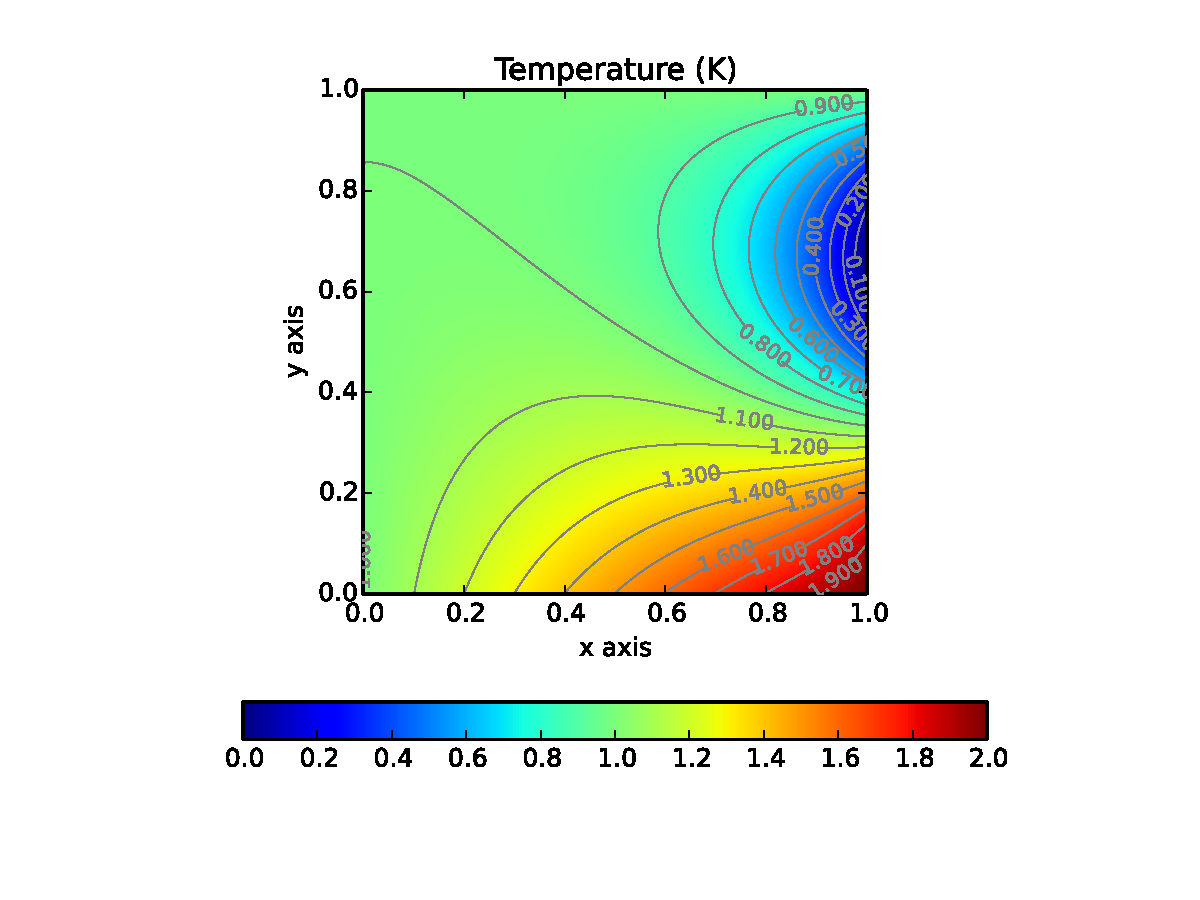
\includegraphics[width=1\linewidth, clip=true, trim = 2cm 1.9cm 2cm .9cm]{simp256}
    \captionof{figure}{Iso-contour plot for T at $\Delta x = \frac{1}{256}$.}
    \label{fig:iso_contour}
\end{figure}
%----------------------------------------------------------------------------------------
%	PART D
%----------------------------------------------------------------------------------------
\section*{d}
\textbf{Using the same boundary conditions of question c, plot $\epsilon_{max}$ versus $\Delta x$ on a set of log-log axes and comment on the form of the plot. Mesh with $\Delta x = \Delta y$, at least 3 different mesh sizes.  Explain how you have decided the minimum $\Delta x = \Delta y$ of your computational domain}

To find the maximum error $\epsilon_{max}$ there are two methods possible:
\begin{itemize}
	\item Calculate analytical solution.
	\item Solve equations using an extremely fine mesh.
\end{itemize}

Whilst for the given problem an analytical solution is possible/feasible to find. Analytical results will not be used, to find $\epsilon_{max}$, as this is not practical for more complex problems.

\subsection*{Grid Independence}
To find an approximation of the true solution a grid independence test is performed. Grid independence occurs when, the solution stops changing or changes very little as the number of elements is increased from $N$ to $2N$. This requires the solutions to have converged, the point at which convergence occurs must be identical between solutions. The point of convergence is said to be when the change in residual $R < 1 \times 10^{-6}$ between two successive iterations. Note that this must be the maximum residual, $R_{max}$ not a mean of the residuals across the entire domain.

\begin{figure}[!htb]
\centering
\begin{subfigure}{.5\textwidth}
  \centering
  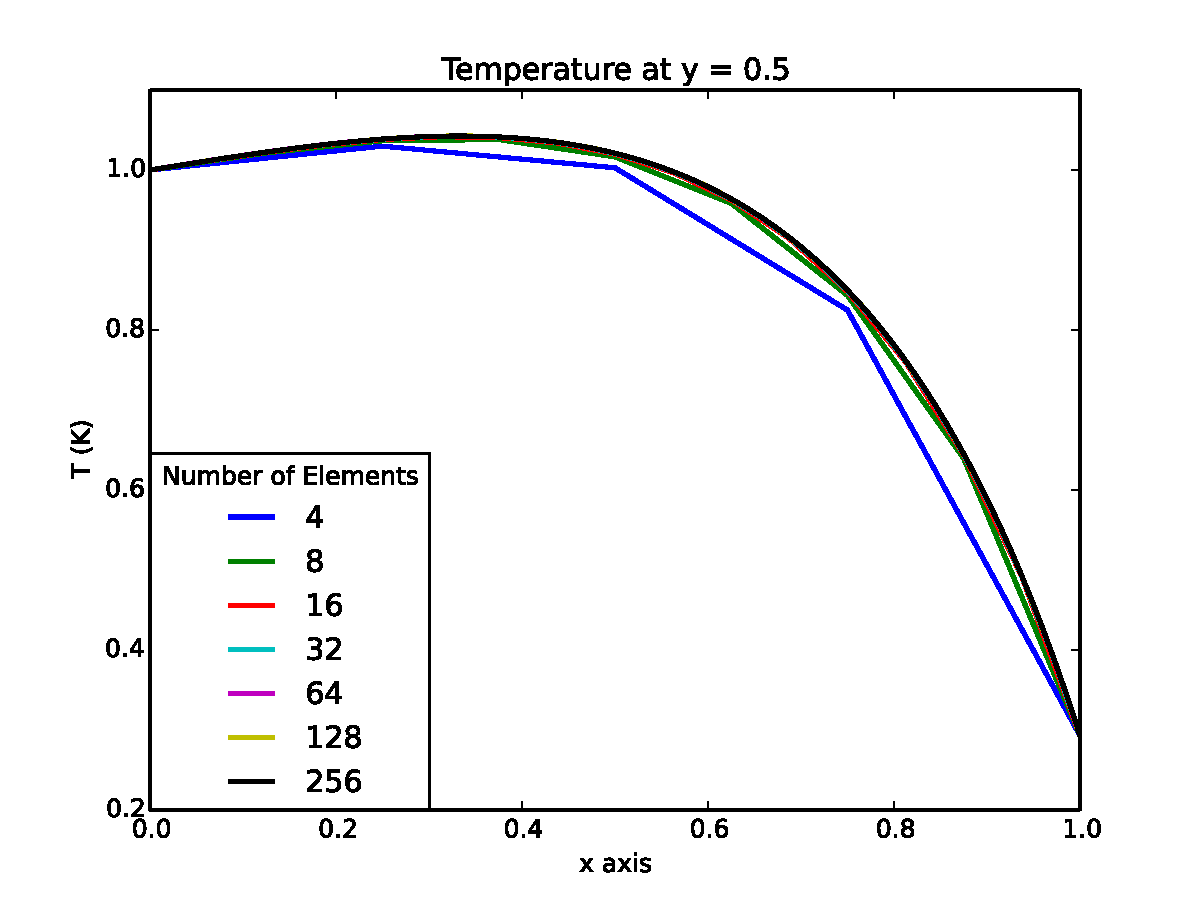
\includegraphics[width=1\linewidth]{grid_ind}
  \caption{Grid Independence Test}
  \label{fig:grid_inda}
\end{subfigure}%
\begin{subfigure}{.5\textwidth}
  \centering
  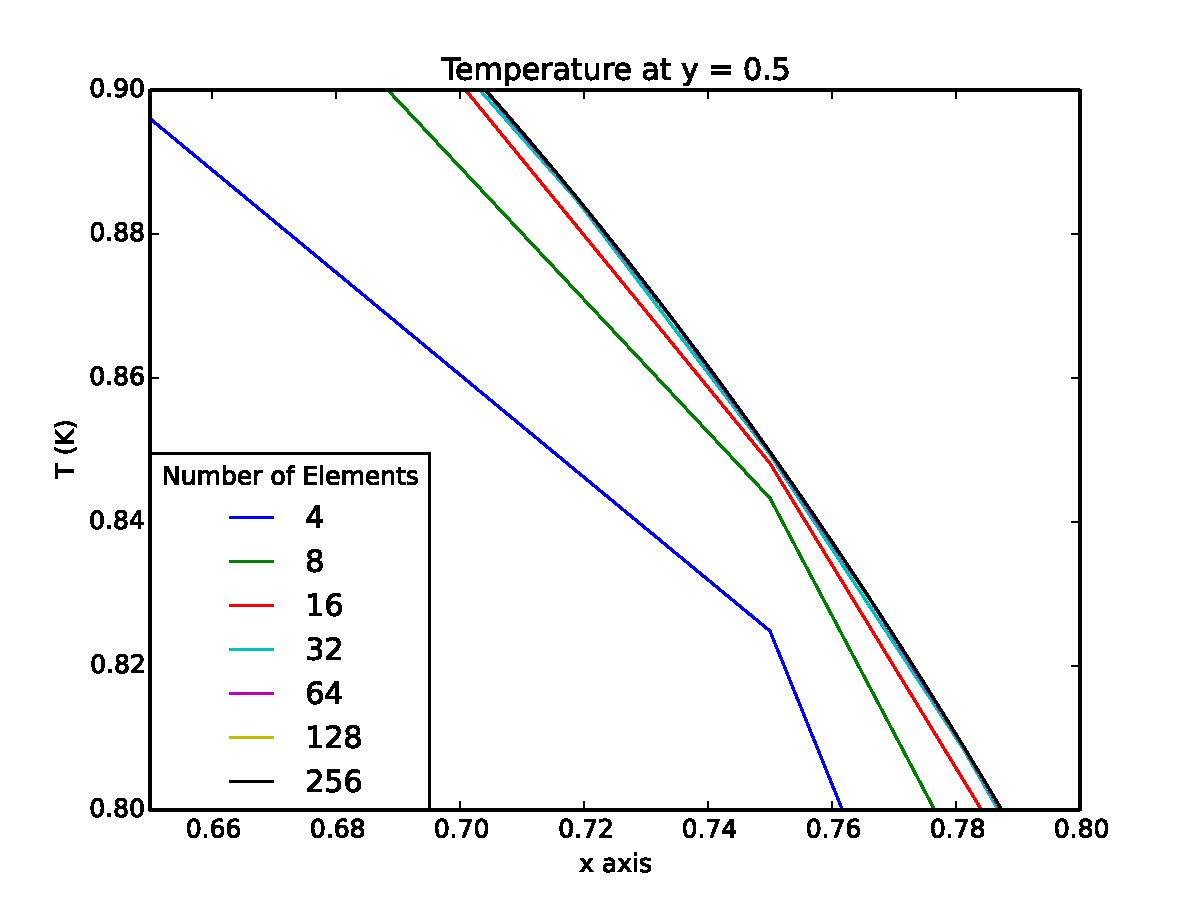
\includegraphics[width=1\linewidth]{grid_zoom}
  \caption{Magnification of Area: (.65,.8)(.8,.9)}
  \label{fig:grid_indb}
\end{subfigure}
\caption{Grid Independence Test.}
\label{fig:grid_ind}
\end{figure}

In figure \ref{fig:grid_ind} we can see a plot of the temperature in Kelvin for the points at $y = 0.5$. As the number of elements are increased the solution tends towards to a final approximation, in figure \ref{fig:grid_inda} almost no difference is seen between $\Delta x = \frac{1}{16}$ and $\Delta x = \frac{1}{256}$. Magnifying the domain slightly, as in figure \ref{fig:grid_indb} it can be seen that there is no pertinent difference in the solution plot as number of elements increases from 64 onwards. Using the solution at $\Delta x = \frac{1}{256}$ we can find the maximum error $\epsilon_{max}$ of the solutions.

The result of $\Delta x = \frac{1}{256}$ is taken as the true solution - $\overline{u}^n$. now the error can be compared between our true approximation, and the solutions given by meshes of varying refinement, for a number of common points across the domain $n$.

\begin{equation}
\epsilon^n = \overline{u}^n - u^n
\end{equation}

\begin{figure}[htb!]
\centering
    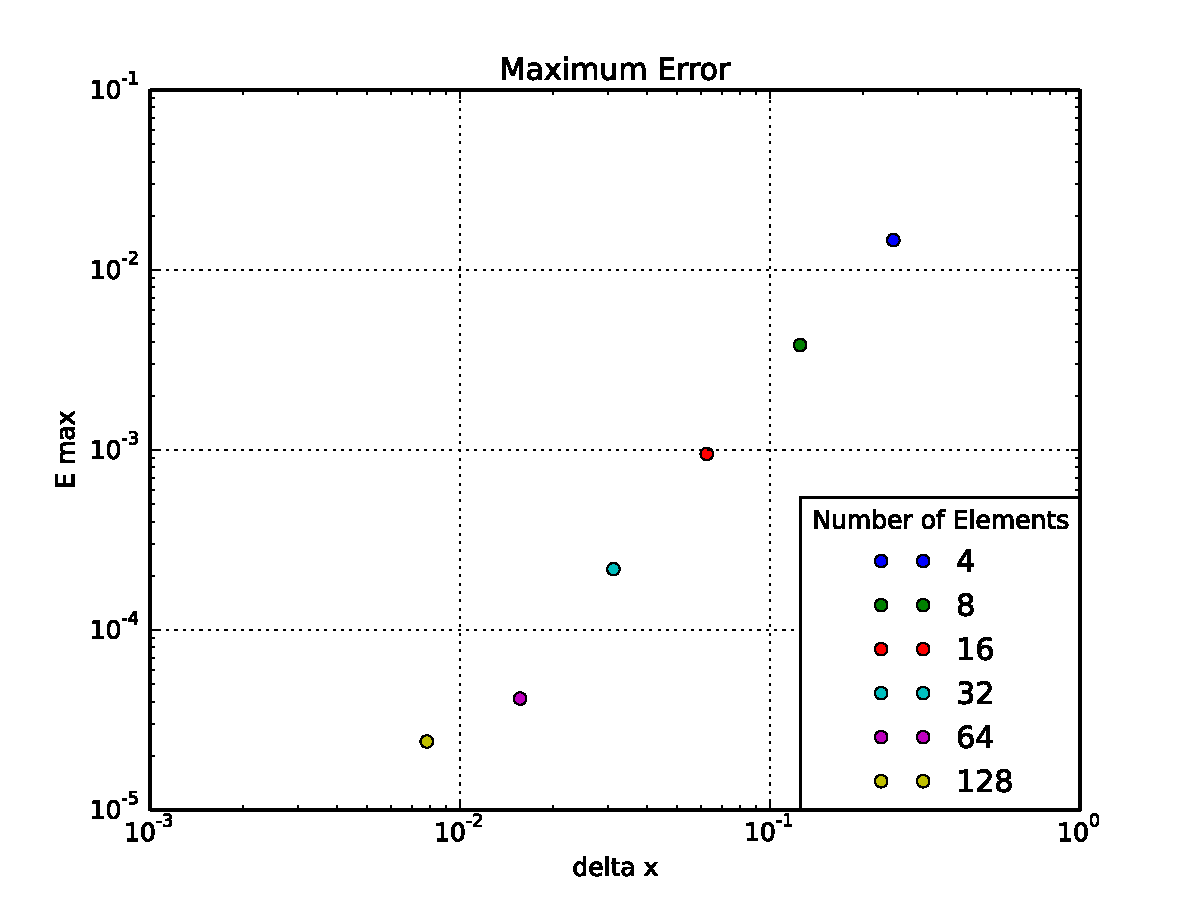
\includegraphics[width=.75\linewidth, clip=true, trim = 0cm 0cm 0cm 0cm]{error}
    \captionof{figure}{Error $\epsilon_{max}$ with change in $\Delta x$.}
    \label{fig:error}
\end{figure}

\begin{center}
\begin{tabular}{| l || c | c |}
  \hline
  $\Delta_x = \Delta_y$ & $\epsilon_{max}$ & Decrease in Error $\%$ \\ \hline
  1/4 & 1.46e-2 & n/a \\
  1/8 & 3.83e-3 & 73.9 \\
  1/16 & 9.52e-4 & 75.2 \\
  1/32 & 2.17e-4 & 77.1 \\
  1/64 & 4.16e-05 & 80.9 \\
  1/128 & 2.40e-05 & 42.3 \\
  \hline
\end{tabular}
\captionof{table}{Error $\epsilon_{max}$ of meshes.}
\label{table:error_change}
\end{center}


In figure \ref{fig:error} the error can be shown as calculated against the converged solution given by mesh $\Delta x = \frac{1}{256}$. Immediately obvious is the linear decrease in error as the mesh size increased. Specifically, as shown in table \ref{table:error_change}, the error is quartered as the mesh size is quadrupled. However this relationship breaks down as the $\Delta x$ becomes less than $\frac{1}{64}$.

The recommendation of $\Delta_x$ for the given problem, using the tested mesh sizes, would to use a $\Delta_x = \Delta_y = \frac{1}{64}$. This size of element gives the most accurate result for the least computational cost.

However using a non-uniform mesh, could save computational cost by increasing the element size in the areas of temperature gradients. Such as the region $0 < x < 0.2$ shown in figure \ref{fig:iso_contour}. Though this is beyond the scope of the coursework presented.

% ---------------------------------------------------------------------------------------
%	BIBLIOGRAPHY
% ---------------------------------------------------------------------------------------
\newpage
\bibliographystyle{unsrt}	% in order of appearance
%\bibliographystyle{acm}	% (uses file "plain.bst")
%\bibliographystyle{abbrv}	% (uses file "plain.bst")
%\bibliographystyle{siam}	% (uses file "plain.bst")
%\bibliographystyle{apalike}
\bibliography{/home/fmg215/Documents/latex/myrefs}		% expects file "myrefs.bib"}
%----------------------------------------------------------------------------------------
% END DOCUMENT
%----------------------------------------------------------------------------------------
\end{document}